
% This LaTeX was auto-generated from MATLAB code.
% To make changes, update the MATLAB code and republish this document.

\documentclass{article}
\usepackage{graphicx}
\usepackage{color}
\usepackage{amsmath}
\usepackage{amssymb}
\usepackage[a4paper, total={6in,8in}]{geometry}
\usepackage{pdfpages}
\usepackage{multicol}

\sloppy
\definecolor{lightgray}{gray}{0.5}
\setlength{\parindent}{0pt}

\begin{document}

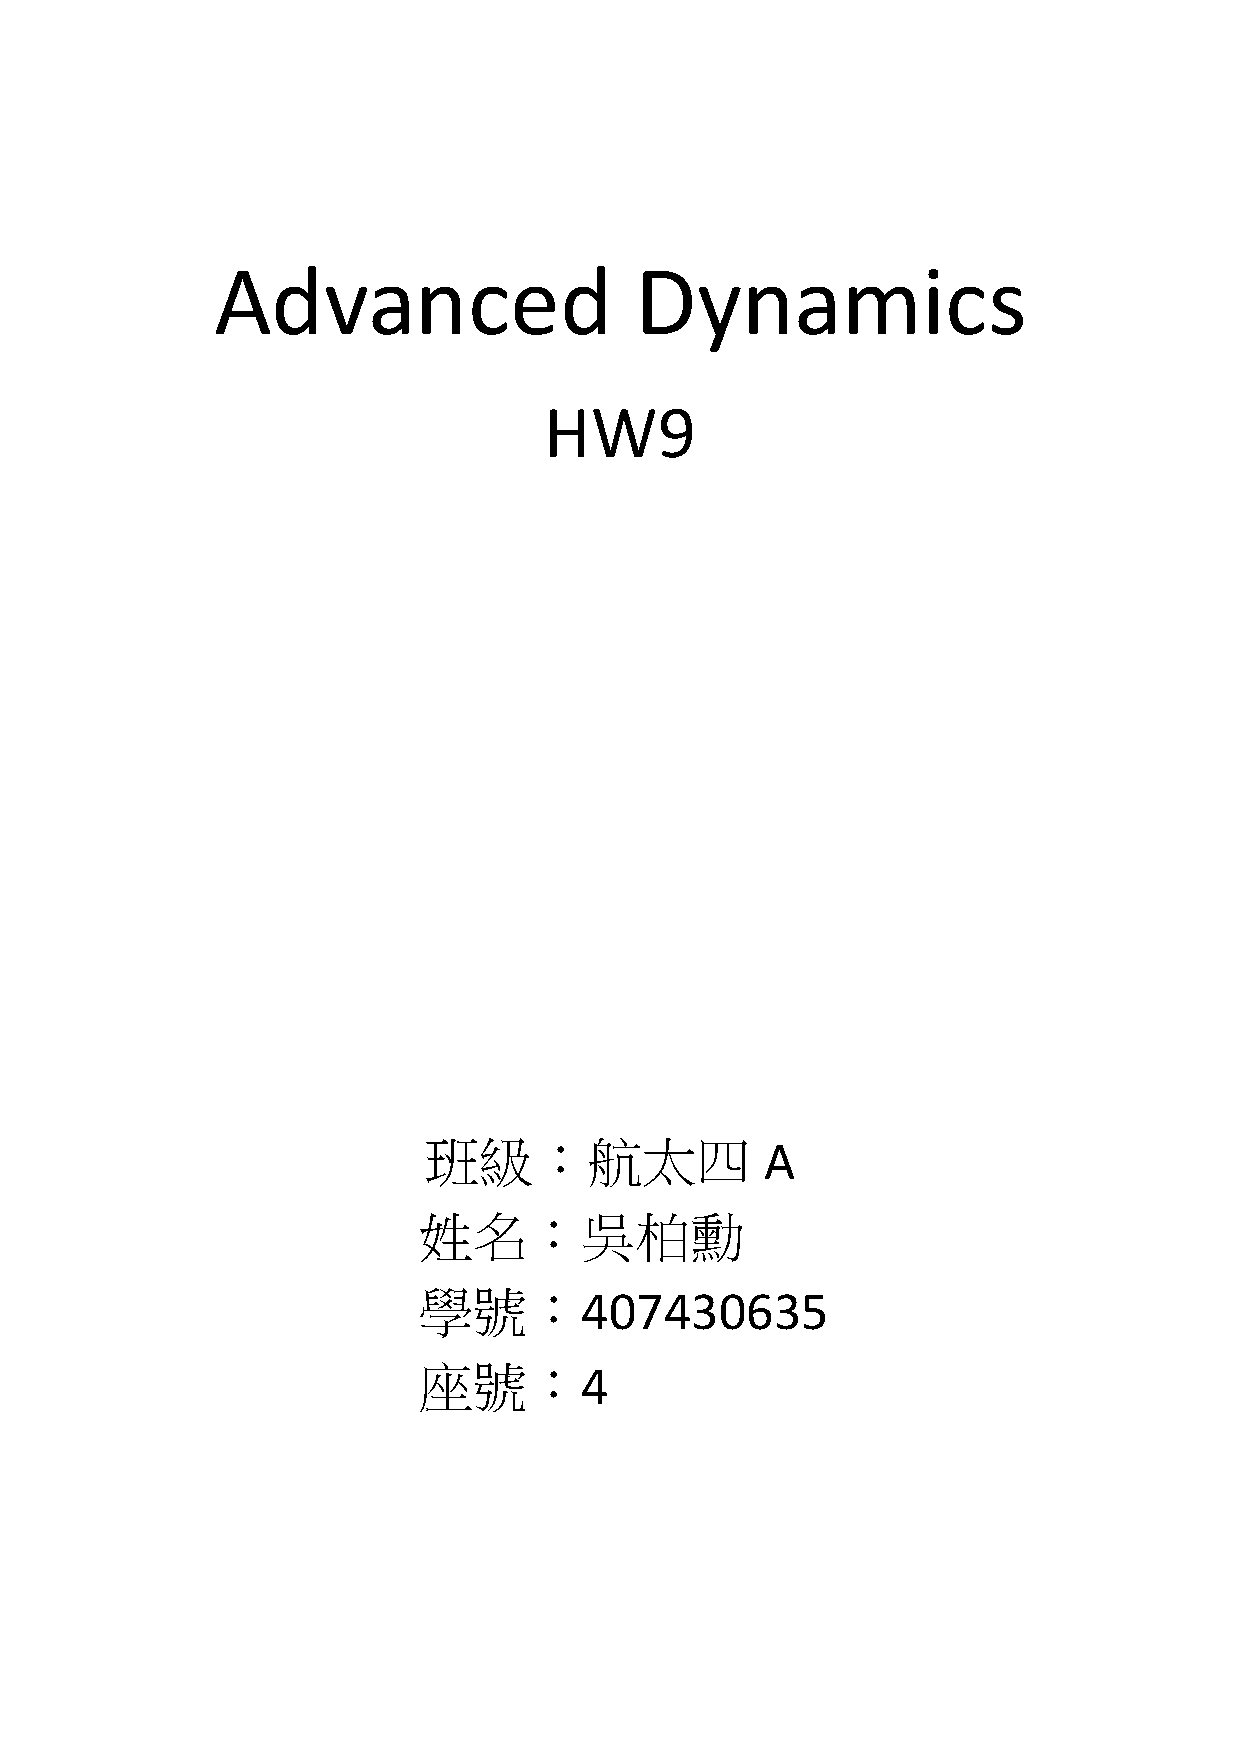
\includepdf{../TitlePage.pdf}

\hrulefill
\subsection*{Formula of motion}



\dotfill
\subsection*{Matlab program}
\begin{verbatim}
clear;clc;close all
syms t r theta omega real
theta = omega*t;
r_C = [r*theta r];
r_Cp = [r*theta 0];
r_Cpp = [r*theta 2*r];
r_M = [r*(theta-sin(theta)) r*(1-cos(theta))];
r_CpM = simplify(r_M-r_Cp);
r_CppM = simplify(r_M-r_Cpp);

v_Cp = simplify(diff(r_Cp, t));
v_M = simplify(diff(r_M, t));
mag_v_M = simplify(sqrt(v_M(1)^2+v_M(2)^2));

DotProduct_r_CpM_v = simplify(dot(r_CpM, v_M));
DotProduct_r_CppM_v = simplify(dot(r_CpM, r_CppM));
fprintf("The dot product between rCpM and v is %s. And it's orthogonal!!! \n", ...
        char(DotProduct_r_CpM_v))
fprintf("The dot product between rCppM and rCpM is %s. And it's orthogonal too!!! \n", ...
        char(DotProduct_r_CppM_v))

a_M = diff(v_M,t);

\end{verbatim}

\dotfill
\subsection*{Program result}
        \color{lightgray} \begin{verbatim}The dot product between rCpM and v is 0. And it's orthogonal!!!
The dot product between rCppM and rCpM is 0. And it's orthogonal too!!!
\end{verbatim} \color{black}


\hrulefill
\subsection*{Calculate the values of the motion}


\dotfill
\subsection*{Matlab program}
\begin{verbatim}
% === Setup some condition ===
tn = 0:0.01:10;
rn = .5;
omegan = 1;
parameters = {tn, rn, omegan};

% === Substitute the condition values to the equation of motion ===
position_M = double(subs(r_M', {t, r, omega}, parameters));
position_C = double(subs(r_C', {t, r, omega}, parameters));
position_Cp = double(subs(r_Cp', {t, r, omega}, parameters));
position_Cpp = double(subs(r_Cpp', {t, r, omega}, parameters));
velocity_M = double(subs(v_M', {t, r, omega}, parameters));
Acceleration_M = double(subs(a_M', {t, r, omega}, parameters));
\end{verbatim}


\hrulefill
\subsection*{Animate of the motion}


\dotfill
\subsection*{Matlab program}
\begin{verbatim}
% Set of the figure config show at below.
% {Show reference, Focus on moving frame, Title of the plot, Set of legend name}
FigureConfig = {{true, true, 'The trajectory of point M focus on the moving frame'},
                {false, false, 'The trajectory of point M focus on the fix frame'}};
% Change the animate play speed
AnimateSpeed = 50;
tspan = 1:AnimateSpeed:length(tn);


for frame = 1:length(FigureConfig)
    figure()
    for i = tspan
        % === Find out the values until the current time ===
        EndPosition_M = position_M(:,i);
        EndPosition_C = position_C(:,i);
        EndPosition_Cp = position_Cp(:,i);
        EndPosition_Cpp = position_Cpp(:,i);
        EndVelocityVector_M = velocity_M(:,i);
        EndAccVector_M = Acceleration_M(:,i);

        % === Reset the current figure ===
        clf

        % === Plot out the figure ===
        hold on; daspect([1 1 1])
        % Plot the trajectory
        plot(position_M(1,1:i), position_M(2,1:i), 'LineWidth', 1.5)
        % Plot the circle
        viscircles(EndPosition_C', rn, 'LineWidth', 1, 'Color', 'k');
        % Draw the velocity vector of point M
        quiver(EndPosition_M(1), EndPosition_M(2), EndVelocityVector_M(1), ...
        EndVelocityVector_M(2), 'LineWidth', 1.5, 'Color', 'r', 'MaxHeadSize', 0.5);
        % Draw the acceleration of point M
        quiver(EndPosition_M(1), EndPosition_M(2), EndAccVector_M(1), EndAccVector_M(2), ...
            'LineWidth', 1.5, 'Color', 'g', 'MaxHeadSize', 0.5);

        % Draw the reference line
        if FigureConfig{frame}{1} == true
            Vector_CpM = {[position_M(1,i) position_Cp(1,i)], ...
                          [position_M(2,i) position_Cp(2,i)]};
            plot(Vector_CpM{1}, Vector_CpM{2}, '--', 'LineWidth', 1.5, 'Color', 'c')
            Vector_CppM = {[position_M(1,i) position_Cpp(1,i)], ...
                           [position_M(2,i) position_Cpp(2,i)]};
            plot(Vector_CppM{1}, Vector_CppM{2}, '--', 'LineWidth', 1.5, 'Color', 'm')
        end

        % Draw the point M
        plot(position_M(1,i), position_M(2,i), '.', 'Color', 'b', 'MarkerSize', 15)
        % Draw the point C
        plot(position_C(1,i), position_C(2,i), '.', 'Color', 'k', 'MarkerSize', 5)

        title(FigureConfig{frame}{3})
        if FigureConfig{frame}{1} == true
            legend('Trajectory', 'Velocity', 'Acceleration', "$\overline{C'M}$", ...
                   "$\overline{C''M}$", 'Point M', 'Point C', 'Interpreter', 'latex')
        else
            legend('Trajectory', 'Velocity', 'Acceleration', 'Point M', ...
                   'Point C', 'Interpreter', 'latex')
        end
        xlabel('x'); ylabel('y')
        if FigureConfig{frame}{2} == true
            % Focus on the point C
            xlim([position_C(1,i)-1 position_C(1,i)+3])
            ylim([-0.5 2])
        else
            xlim([-1 7])
            ylim([-1 4])
        end
        grid()
        drawnow
    end
end
\end{verbatim}

\dotfill
\subsection*{Program result}

\begin{par}
From Figure 1, we can know that the result in the first section was correct. $\overline{C^{'}M}$ was orthogonal with $\textbf{v}$, and $\overline{C^{''}M}$ was orthogonal with $\overline{C^{'}M}$ too.
\end{par}

\begin{figure*}[h]
    \centering
    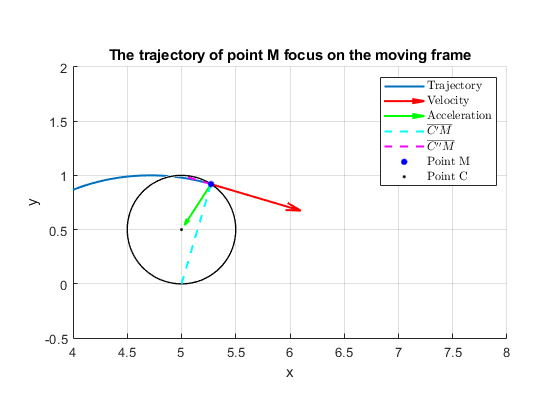
\includegraphics [width=5in]{HW3_01.png}
    \caption{The trajectory of point M on the moving frame}
\end{figure*}

\begin{figure*}[h]
    \centering
    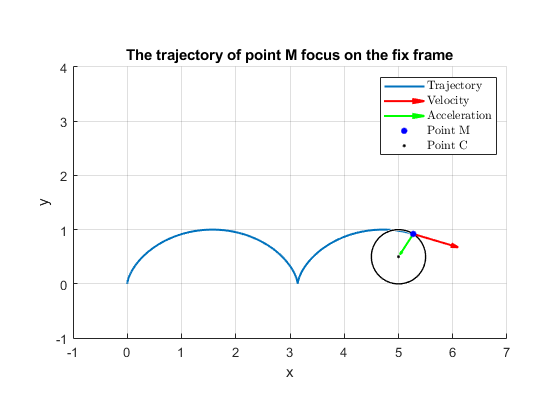
\includegraphics [width=5in]{HW3_02.png}
    \caption{The trajectory of point M on the fix frame}
\end{figure*}


\end{document}

